\documentclass{beamer}
\usetheme{Frankfurt}
\usepackage[style=ieee,maxbibnames=3,minbibnames=1]{biblatex}
\usepackage{tikz}
\usetikzlibrary{shapes.geometric, arrows}

\addbibresource{lecture.bib}
\addtobeamertemplate{navigation symbols}{}{%
    \usebeamerfont{footline}%
    \usebeamercolor[fg]{footline}%
    \hspace{1em}%
    \insertframenumber/\inserttotalframenumber
}

\setbeamertemplate{bibliography item}{\insertbiblabel}
\title{Developing an Autonomous Vehicle}
\subtitle{A Use-Case in Software Engineering}
\author{Dr. Michael Aeberhard}
\institute{Apex.AI}
\date{February 7, 2021}
\logo{\includegraphics[height=0.5cm]{images/tum.png}}

\begin{document}

\frame{\titlepage}

\section{introduction}

\section{Introduction}

% About me
\begin{frame}[t]
\frametitle{About Me}
\framesubtitle{Education}
\begin{columns}[T]
    \begin{column}{.80\textwidth}
    \begin{itemize}
        \item Georgia Institue of Technology (2002-2009)
        \begin{itemize}
            \item B.S. in Computer Engineering (2007)
            \item M.S. in Electrical Engineering (2009)
            \item Formula Student, BMW Motorsport, BMW Plant Spartanburg
        \end{itemize}
        \item CentraleSup\'{e}lec, Master Professionelle (2009)
        \begin{itemize}
            \item Master Thesis @ Daimler AG - \emph{Processing of Out-of-Sequence
                Measurements in Tracking for an Automotive Pre-Crash Application}
        \end{itemize}
        \item Technische Universit\"{a}t Dortmund, Dr.-Ing. (2010-2017)
        \begin{itemize}
            \item Dissertation: \emph{\href{https://eldorado.tu-dortmund.de/handle/2003/36011}{Object-level fusion for surround environment perception in automated driving applications}}
            \item In cooperation with BMW AG
        \end{itemize}
    \end{itemize}
    \end{column}
    \begin{column}{.20\textwidth}
    \centering
    \includegraphics[height=2.0cm]{images/michael-aeberhard-profile.jpg} \\
    \end{column}
\end{columns}
\end{frame}

\begin{frame}
\frametitle{About Me}
\framesubtitle{Career}
\begin{columns}[T]
    \begin{column}{.70\textwidth}
    \begin{itemize}
        \item BMW AG (2010-2018)
        \begin{itemize}
            \item Research in sensor data fusion
            \item Involved in German/EU funded reserach projects:
                SmartSenior, UR:BAN, AdaptIVe
            \item Developer, Product Owner, Project Lead for autonomous driving
        \end{itemize}
        \item Autonomus Intelligent Driving GmbH (2018-2020)
        \begin{itemize}
            \item Developer and Tech Lead for L4 "robot taxi" application
        \end{itemize}
        \item \href{https://www.apex.ai/}{Apex.AI} (2020-)
        \begin{itemize}
            \item Head of Application Engineering
            \item Bringing a safety-certified version ROS 2 to series production
        \end{itemize}
    \end{itemize}
    \end{column}
    \begin{column}{.30\textwidth}
    \centering
    \includegraphics[height=2.0cm]{images/michael-aeberhard-bmw.jpg} \\
    \tiny \copyright \, 2013 BMW AG
    \end{column}
\end{columns}
\end{frame}
\begin{frame}
\frametitle{History of Autonomous Vehicles Development}
\framesubtitle{The Early Years (1990s)}
\begin{columns}[T]
    \begin{column}{.5\textwidth}
    \centering
    Prometheus Project \\
    \vspace{0.25cm}
    \includegraphics[height=2.2cm]{images/vamp.jpg} \\
    \tiny{\cite{Dickmanns1994} VaMP}
    \footnotesize
    \begin{itemize}
        \item European R\&D project (1985 - 1995)
        \item Prof. Ernst Dickmann's research vehicles
            demonstrated 1,000+ km automated highway drives
    \end{itemize}
    \end{column}
    \pause
    \begin{column}{.5\textwidth}
    \centering
    Demo '97 \\
    \vspace{0.25cm}
    \includegraphics[height=2.2cm]{images/demo-97-no-hands.png} \\
    \tiny{Platoon demo}\footnotemark[1]
    \footnotesize
    \begin{itemize}
        \item US DOT sponsored research to demonstrate the
            Automated Highway System (AHS)
        \item A 12 km stretch of an HOV lane was used for the demonstration
    \end{itemize}
    \end{column}
\end{columns}
\pause
\footnotesize
\begin{block}{}
These projects set the foundation for OEM ADAS development in the
2000s
\end{block}
\footnotetext[1]{\tiny{\url{https://path.berkeley.edu/research/connected-and-automated-vehicles/national-automated-highway-systems-consortium}}}
\end{frame}

\begin{frame}
\frametitle{History of Autonomous Vehicles Development}
\framesubtitle{The DARPA Challenges (2004-2008)}
\begin{columns}[T]
    \begin{column}{.65\textwidth}
    DARPA Grand Challenges\footnotemark[1]
    \begin{itemize}
        \item In the 2004 competition, 15 teams competed for a \$1 million prize
            on a 240 km desert route
        \item The prize went unclaimed; the best team was able to complete
            11.78 km
        \item In 2005, a \$2 million prize was up for grabs on a 212 km route
        \item The team from Stanford University with their vehicle
            \emph{Stanley} completed the course the fastest (in total 5 teams
            completed the course)
    \end{itemize}
    \end{column}
    \begin{column}{.35\textwidth}
    \centering
    \includegraphics[height=3cm]{images/darpa_stanley.jpg} \\
    \tiny{\cite{DARPAStanley}}
    \end{column}
\end{columns}
\footnotetext[1]{\tiny{\url{https://www.darpa.mil/about-us/timeline/-grand-challenge-for-autonomous-vehicles}}}
\end{frame}
    
\begin{frame}
\frametitle{History of Autonomous Vehicles Development}
\framesubtitle{The DARPA Challenges (2004-2008)}
\begin{columns}[T]
    \begin{column}{.6\textwidth}
    DARPA Urban Challenge\footnotemark[1]
    \begin{itemize}
        \item In 2007, a third competition for a \$2 million prize was held on
            a 96 km urban route
        \item A total of 11 teams competed in the final competition
        \item A team from Carnegie Melon University won with their vehicle
            \emph{Boss}
    \end{itemize}
    \end{column}
    \begin{column}{.4\textwidth}
    \centering
    \includegraphics[height=3cm]{images/darpa_boss.jpg} \\
    \tiny{\cite{CMUUrbanChallenge}}
    \end{column}
\end{columns}
\pause
\vspace{0.25cm}
\begin{block}{}
The student, engineers, and companies of the DARPA challenges laid the
foundations for today's autonomous driving development and are leaders in the
industry.
\end{block}
\footnotetext[1]{\tiny{\url{https://www.darpa.mil/about-us/timeline/darpa-urban-challenge}}}
\end{frame}

\begin{frame}
\frametitle{History of Autonomous Vehicles Development}
\framesubtitle{The Industry Ramp-Up Phase (2010-2020)}
\centering OEMs and Tier 1s
\begin{columns}[T]
    \begin{column}{.25\textwidth}
        \centering
        \includegraphics[height=1.9cm]{images/bmw_had.jpg} \\
        \footnotesize BMW \cite{AeberhardBMWHAF2015}
    \end{column}
    \begin{column}{.25\textwidth}
        \centering
        \includegraphics[height=1.9cm]{images/mercedes_bertha_benz_drive.jpg} \\
        \footnotesize Mercedes-Benz \cite{DaimlerBertha2014}
    \end{column}
    \begin{column}{.25\textwidth}
        \centering
        \includegraphics[height=1.9cm]{images/bosch_had.jpg} \\
        \footnotesize Bosch \cite{BoschPressHAD}
    \end{column}
    \begin{column}{.25\textwidth}
        \centering
        \includegraphics[height=1.9cm]{images/continental_had.jpg} \\
        \footnotesize Continental \cite{ContinentalHAD}
    \end{column}
\end{columns}
\vspace{0.5cm}
\centering New Players
\begin{columns}[T]
    \begin{column}{.25\textwidth}
        \centering
        \includegraphics[height=1.9cm]{images/waymo_firefly.jpg} \\
        \footnotesize Waymo \cite{WaymoPress}
    \end{column}
    \begin{column}{.25\textwidth}
        \centering
        \includegraphics[height=1.9cm]{images/cruise_vehicle.jpg} \\
        \footnotesize Cruise \cite{CruiseNews}
    \end{column}
    \begin{column}{.25\textwidth}
        \centering
        \includegraphics[height=1.9cm]{images/zoox_vehicle.jpg} \\
        \footnotesize Zoox \cite{ZooxPress}
    \end{column}
    \begin{column}{.25\textwidth}
        \centering
        \includegraphics[height=1.9cm]{images/tusimple_vehicle.jpg} \\
        \footnotesize TuSimple \cite{TuSimpleMedia}
    \end{column}
\end{columns}
\end{frame}

\begin{frame}
\frametitle{History of Autonomous Vehicles Development}
\framesubtitle{Going to Production (2020 - ???)}
Only since 2020 have the first true driveless vehicles been allowed to operate
on public roads, albeit in limited numbers and locations.\\
\begin{columns}[]
    \begin{column}{0.5\textwidth}
        \centering
        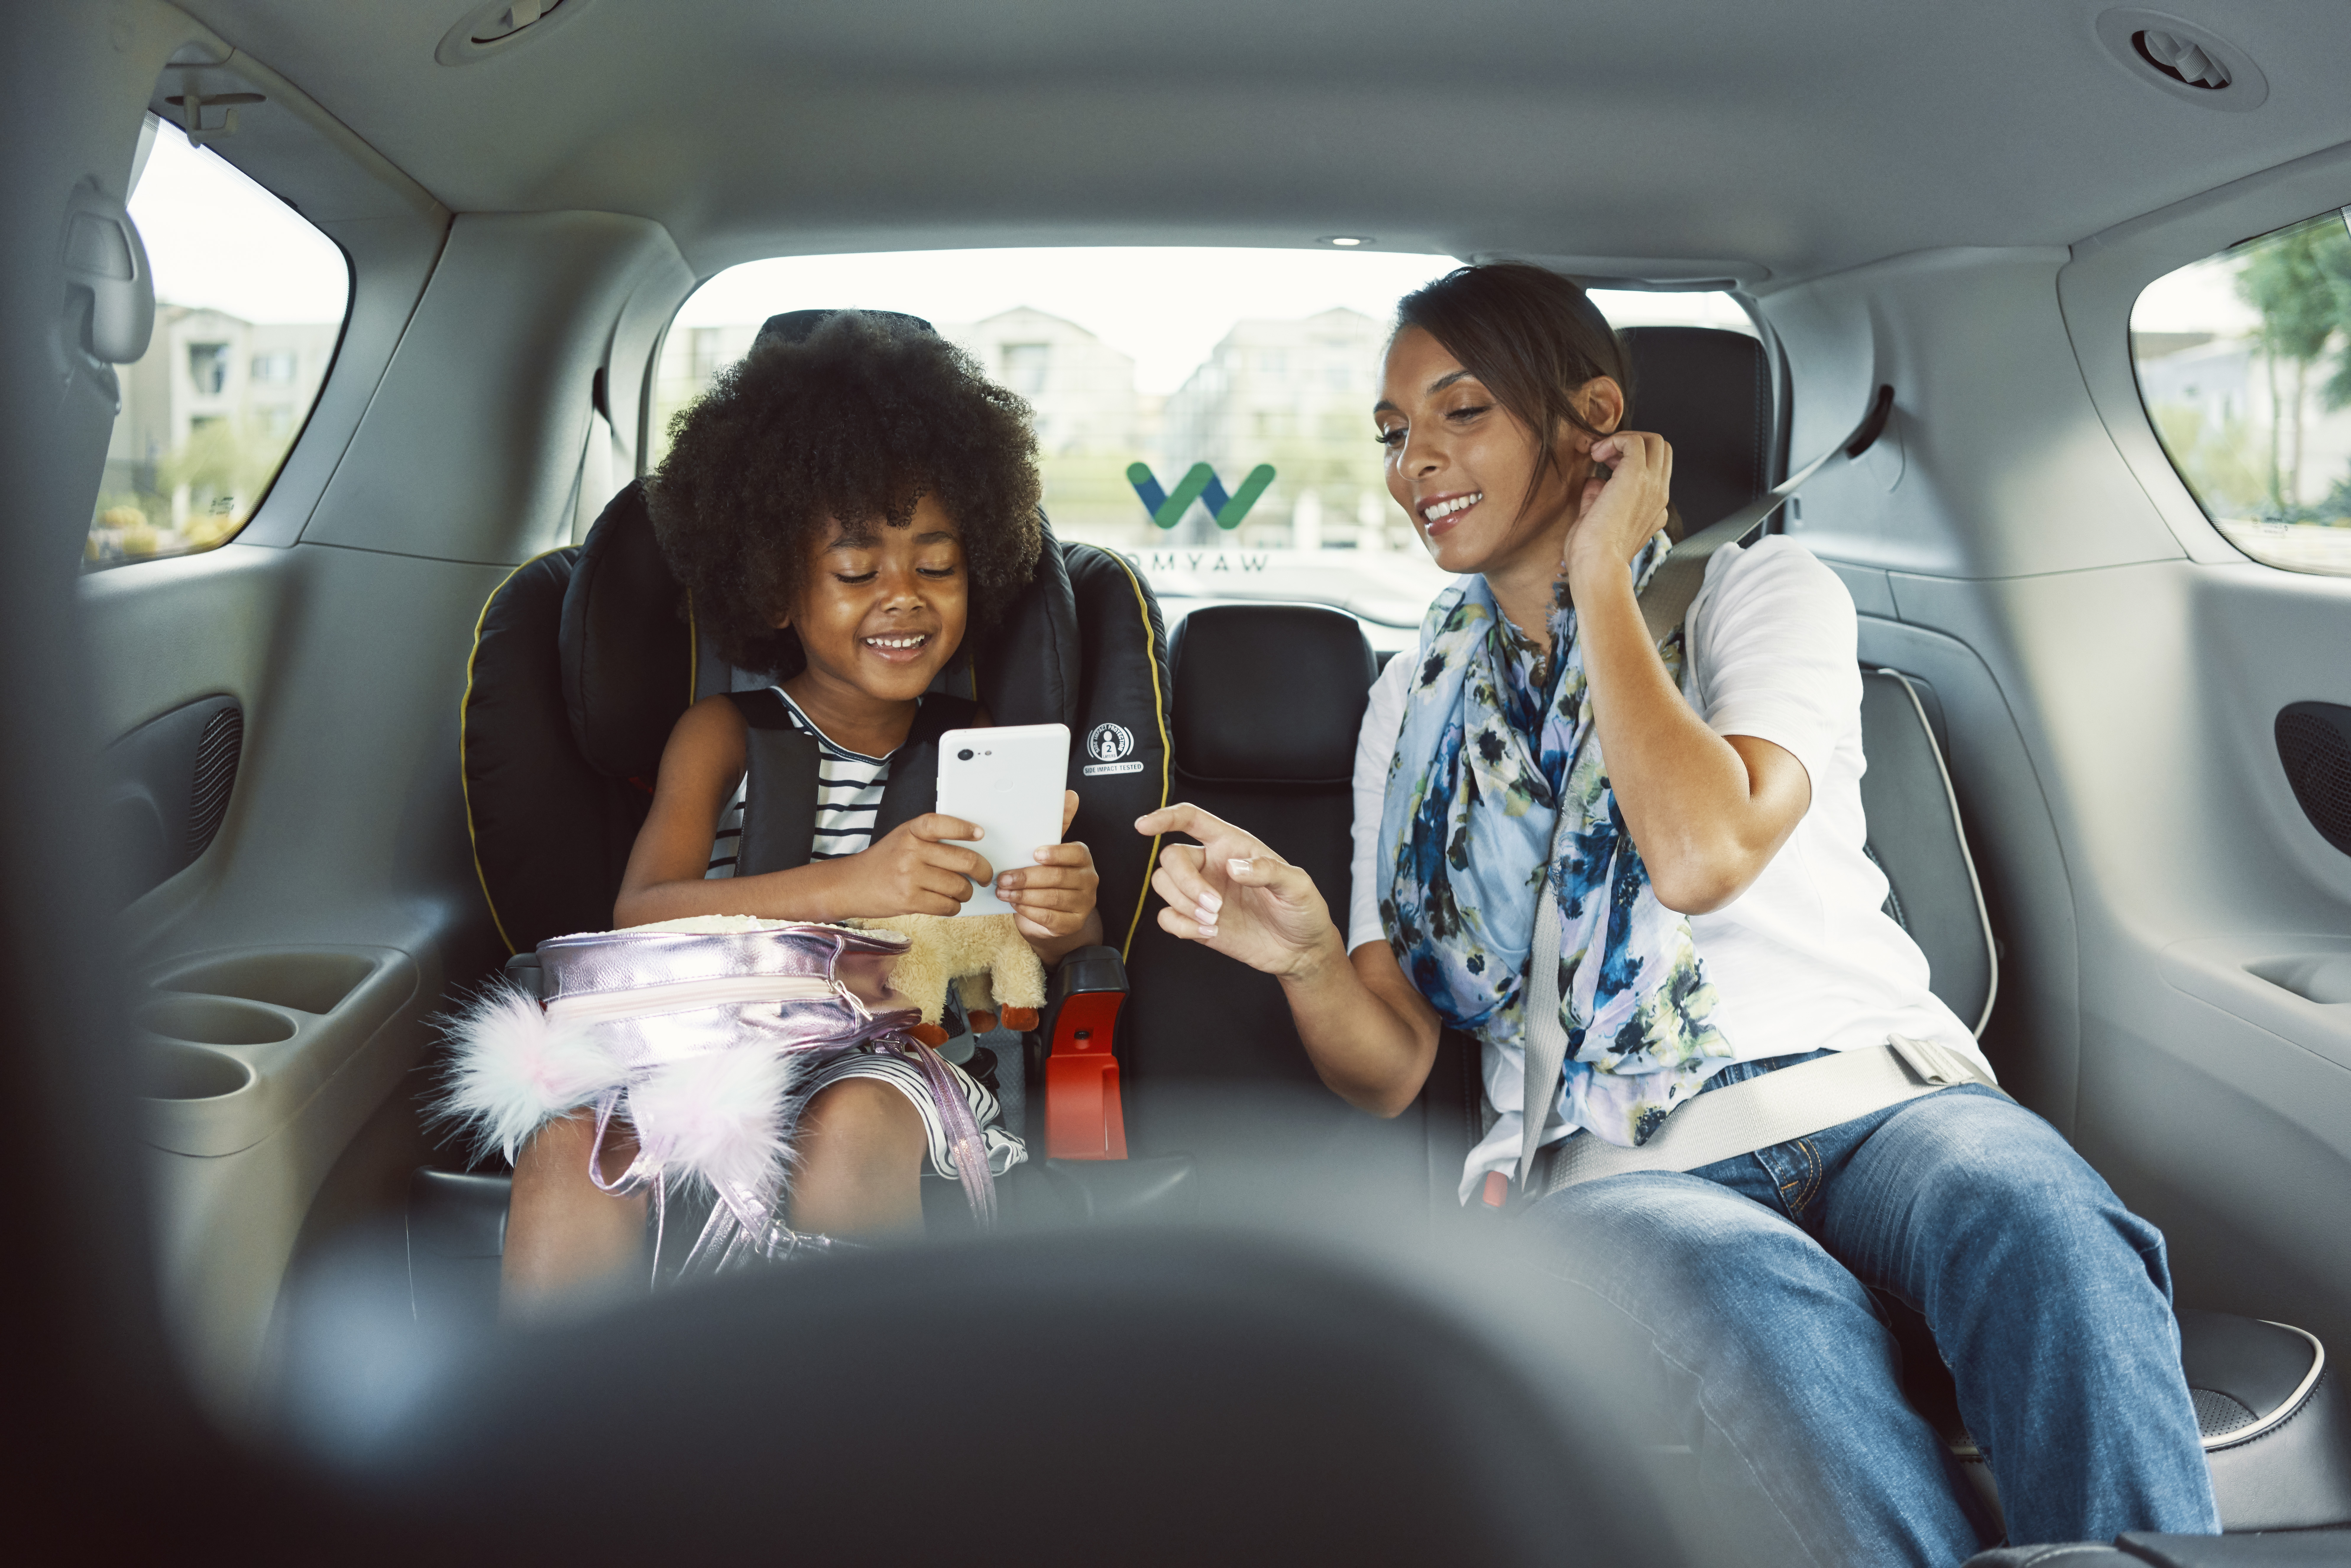
\includegraphics[height=2.5cm]{images/waymo_one.jpg} \\
        \footnotesize Waymo One\footnotemark[1]
    \end{column}
    \begin{column}{0.5\textwidth}
        \centering
        \includegraphics[height=2.5cm]{images/mercedes-level-3.jpg} \\
        \footnotesize Mercedes-Benz DRIVE PILOT \cite{MercedesLevel3}
    \end{column}
\end{columns}
\begin{block}{}
The next decade will be the beginning of the commercialization of autonomous
vehicles. Many challenges remain for widespread adoption...
\end{block}
\footnotetext[1]{\tiny{\url{https://waymo.com/waymo-one/}}}
\end{frame}

\begin{frame}
\frametitle{The Software Challenge}
Modern vehicles are smartphones on wheels and the next generation vehicles
will automated the driving task.\\
$\Rightarrow$ Software is taking over the automotive industry
\vspace{0.25cm}
\begin{itemize}
    \item Dozens of ECUs in a modern vehicle
    \item High-resolution displays for the drive and passenger
    \item Sensors detect the vehicle's environment
    \item Actuators automatically control many vehicle functions
    \item Thousands of software developers from many companies collaborating
    \item Safety of utmost importance
\end{itemize}
\end{frame}

\begin{frame}
\frametitle{The Software Challenge}
\framesubtitle{Autonomous Driving}
Show that the translation of input to output is done with software
\end{frame}

\begin{frame}
\frametitle{The Phases of Development}
Autonomous vehicles and ADAS development has traditionally followed three phases
of development.

\begin{itemize}
    \item Research: Develop prototypes to understand the use-cases, algorithms,
        hardware, etc. $\rightarrow$ is the product feasible?
    \item Pre-development: Iron out the details, requirements, commercial
        viability, etc. $\rightarrow$ develop a solid blue print for production
    \item Production: Software and hardware is hardened and optimized for
        production quality and cost, meeting any required safety, automotive or
        product standards
\end{itemize}
\begin{block}{}
The autonomous driving industry today is making the transition from
pre-development to production.
\end{block}
\end{frame}

\section{Architecture}

\begin{frame}
\frametitle{Architecture}
The architecture of a system can be broken down into different levels of
detail.

TODO: Show as a pyramid or layered picture?

\begin{itemize}
    \item Functional Architecture: Logical components and sub-systems, along
        with a high-level definition of interfaces, are identified
    \item Software Architecture: Implementation of logical components into
        concrete software components with concrete interface implementations
    \item Hardware Architecture: Partitioning of the software components onto
        specific hardware and defining the low-level communication mechanisms
        of the components
\end{itemize}

The different phases of development will focus on different levels of
the architecture and hence specific details of the system.
\end{frame}

\subsection{Functional Architecture}

\begin{frame}
\frametitle{Functional Architecture}
The functional architecture is initially developed during the research phase
and refined as development matures to production.

\begin{itemize}
    \item The main components of a system are identified
    \item Specific algorithms which realize the components are developed
    \item High-level interfaces between components are created
\end{itemize}

\begin{block}{}
The functional architecture for an autonomous driving vehicle has evolved
over the past decade and is converging towards an industry standard.
\end{block}
\end{frame}

\begin{frame}
\frametitle{Sense - Plan - Act}
\framesubtitle{Common Autonomous Vehicle Functional Architecture}
The \emph{Sense - Plan - Act} architecture is still predominant in modern autonomous
vehicle architectures.

\vspace{1cm}

\begin{center}
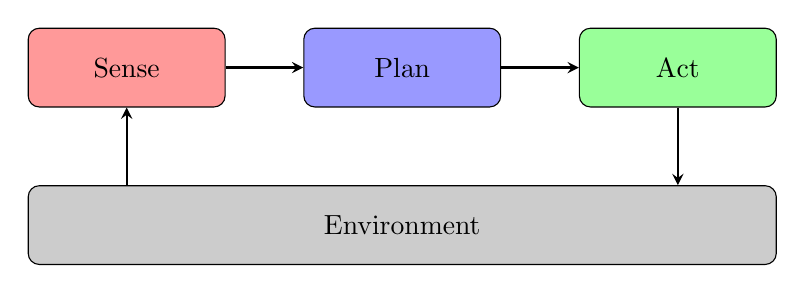
\begin{tikzpicture}[node distance=3.5cm]
    \node (sense)[rectangle,rounded corners,minimum width=2.5cm,minimum height=1cm,text centered,draw=black,fill=red!40]{Sense};
    \node (plan)[right of=sense,rectangle,rounded corners,minimum width=2.5cm,minimum height=1cm,text centered,draw=black,fill=blue!40]{Plan};
    \node (act)[right of=plan,rectangle,rounded corners,minimum width=2.5cm,minimum height=1cm,text centered,draw=black,fill=green!40]{Act};
    \node (environment)[below of=plan,yshift=1.5cm,rectangle,rounded corners,minimum width=9.5cm,minimum height=1cm,text centered,draw=black,fill=gray!40]{Environment};
    \draw [thick,->,>=stealth] (sense) -- (plan);
    \draw [thick,->,>=stealth] (plan) -- (act);
    \draw [thick,->,>=stealth] (act) -- ([xshift=3.5cm]environment.north);
    \draw [thick,<-,>=stealth] (sense) -- ([xshift=-3.5cm]environment.north);
    \end{tikzpicture}
\end{center}
\end{frame}

\begin{frame}
\frametitle{Sense - Plan - Act}
\framesubtitle{Common Autonomous Vehicle Functional Architecture}
\includegraphics[width=\textwidth]{images/tas_2016_fig4_av_functional_architecture.png}
\tiny{Architecture image from \cite{Tas2016-sd} based on the vehicle that won the
Korean Autonomous Vehicle Competition \cite{Jo2014-na}}.
\end{frame}

\begin{frame}
\frametitle{Sensors}
Autonomous vehicles use a combination of cameras, radar and lidar sensors to
sense and perceive the environment. \\
\vspace{0.5cm}
\includegraphics[width=\textwidth]{images/waymo_sensors.png}
\footnotesize{Waymo sensor suite\footnotemark[1]}
\footnotetext[1]{\tiny{\url{https://blog.waymo.com/2020/03/introducing-5th-generation-waymo-driver.html}}}
\end{frame}

\begin{frame}
\frametitle{Sensors}
\framesubtitle{Camera}
\begin{columns}[T]
    \begin{column}{.5\textwidth}
        \centering
        \includegraphics[height=2.0cm]{images/daimler_cameras.jpg}\\
        \tiny{Source: Daimler\footnotemark[1]}
    \end{column}
    \begin{column}{.5\textwidth}
        \centering
        \href{https://www.youtube.com/watch?v=rACZACXgreQ}{
        \includegraphics[height=2.0cm]{images/tesla_autopilot_cameras.jpg}}\\
        \tiny{Tesla camera system, Source: YouTube (greentheonly)\footnotemark[2]}
    \end{column}
\end{columns}

\vspace{0.2cm}

\footnotesize
Vision sensors are the basis for an autonomous driving system, providing
important perception input for many different purposes.

\begin{columns}[T]
    \begin{column}{0.45\textwidth}
        \footnotesize
        Capabilities:
        \begin{itemize}
            \item Dynamic object detection
            \item Static object detection
            \item Lane and road detection
            \item Classification
            \item Traffic sign/light detection
        \end{itemize}
    \end{column}
    \begin{column}{0.55\textwidth}
        \footnotesize
        Important properties:
        \begin{itemize}
            \item High dynamic range
            \item $360\deg$ field of view
            \item Global shutter
            \item Low cost
            \item No distance or velocity measurements
        \end{itemize}
    \end{column}
\end{columns}

\footnotetext[1]{\tiny{\url{https://www.daimler.com/magazine/technology-innovation/automation-daimler-immendingen-camera-radar-lidar.html}}}
\footnotetext[2]{\tiny{\url{https://www.youtube.com/watch?v=rACZACXgreQ}}}
\end{frame}

\begin{frame}
\frametitle{Sensors}
\framesubtitle{Radar}
\begin{columns}[b]
    \begin{column}{.5\textwidth}
        \centering
        \includegraphics[height=2.0cm]{images/continental_radar.jpg}\\
        \vspace{0.2cm}
        \tiny{Source: Continental\footnotemark[1]}
    \end{column}
    \begin{column}{.5\textwidth}
        \centering
        \includegraphics[height=2.5cm]{images/daimler_radar_dataset.png}\\
        \tiny{Source: Daimler, RadarScene dataset\footnotemark[2]}
    \end{column}
\end{columns}

\vspace{0.2cm}

\footnotesize
Radar has been the workhorse of ADAS for over two decades, being the main
sensor for ACC and continues its importance in autonomous driving systems.

\begin{columns}[T]
    \begin{column}{0.4\textwidth}
        \footnotesize
        Capabilities:
        \begin{itemize}
            \item Dynamic object detection
            \item Static object detection
            \item Road boundary detection
        \end{itemize}
    \end{column}
    \begin{column}{0.6\textwidth}
        \footnotesize
        Important properties:
        \begin{itemize}
            \item Robust in weather, e.g. rain, fog, etc.
            \item Direct measurement of speed
            \item Reasonable cost
            \item Low resolution, poor vertical separation
        \end{itemize}
    \end{column}
\end{columns}
\footnotetext[1]{\tiny{\url{https://www.continental-automotive.com/en-gl/Passenger-Cars/Autonomous-Mobility/Enablers/Radars/Long-Range-Radar/ARS540}}}
\footnotetext[2]{\tiny{\url{https://radar-scenes.com/}}}
\end{frame}

\begin{frame}
\frametitle{Sensors}
\framesubtitle{Lidar}
\begin{columns}[T]
    \begin{column}{.5\textwidth}
        \centering
        \includegraphics[height=2.5cm]{images/velodyne_lidars.png}\\
        \tiny{Source: Velodyne\footnotemark[1]}
    \end{column}
    \begin{column}{.5\textwidth}
        \centering
        \includegraphics[height=2.5cm]{images/velodyne_pointcloud.jpg}\\
        \tiny{Source: Velodyne\footnotemark[1]}
    \end{column}
\end{columns}

\vspace{0.2cm}

\footnotesize
Only very recently has lidar been introduced in production vehicles, but it has
been a core sensor of autonomous driving research since the DARPA challenges.

\begin{columns}[T]
    \begin{column}{0.4\textwidth}
        \footnotesize
        Capabilities:
        \begin{itemize}
            \item Dynamic and static object detection
            \item Road boundary and curb detection
            \item Lane detection
        \end{itemize}
    \end{column}
    \begin{column}{0.6\textwidth}
        \footnotesize
        Important properties:
        \begin{itemize}
            \item High resolution
            \item Large field of view
            \item Measure intensity
            \item Poor weather robustness
            \item No velocity measurement
        \end{itemize}
    \end{column}
\end{columns}
\footnotetext[1]{\tiny{\url{https://velodynelidar.com/media-kit/}}}
\end{frame}

\begin{frame}
\frametitle{Perception}
\framesubtitle{Object Detection and Tracking}

\end{frame}

\begin{frame}S
\frametitle{Perception}
\framesubtitle{Occupancy Grids}

\end{frame}

\begin{frame}
\frametitle{Perception}
\framesubtitle{Sensor Data Fusion}

\end{frame}

\begin{frame}
\frametitle{Localization}

\end{frame}

\begin{frame}
\frametitle{Prediction}

\end{frame}

\begin{frame}
\frametitle{Motion Planning}

\end{frame}

\begin{frame}
\frametitle{Vehicle Control}

\end{frame}

\begin{frame}
\frametitle{Machine Learning in Autonomous Driving}

\end{frame}

\subsection{Software Architecture}

\begin{frame}
\frametitle{Software Architecture}
Show layered architecture, e.g. HW, OS, Middleware, Framework, Apps
\end{frame}

\begin{frame}
\frametitle{Software Architecture}
Talk about how functional components are implemented into software:
AUTOSAR, ROS, etc.

Talk also about the development tools required to implement a software 
architecture
\end{frame}

\begin{frame}
\frametitle{Prototyping in the ROS Framework}
Talk about how a prototyping framework like ROS is useful
\end{frame}

\begin{frame}
\frametitle{Production Software Frameworks}
Talk about how what is required to go from prototyping to a production
software architecture (Apex.OS, AUTOSAR, other --> name the properties
of such frameworks)
\end{frame}

\subsection{Hardware Architecture}

\begin{frame}
\frametitle{Hardware Architecture}
\framesubtitle{Early prototyping}
Early research and pre-development phases of development are able to
implement a working system using off-the-shelf PC-like Hardware
(e.g. x86 architecture with Linux).

TODO: Show example of such hardware in a prototype vehicle
\end{frame}

\begin{frame}
\frametitle{Hardware Architecture}
\framesubtitle{Early Embedded Hardware}
Talk about what early embedded hardware looks like, e.g. evaluation boards,
etc. --> also mentioned starting to go to microcontrollers, if required, or
RTOS. Give examples with pictures.
\end{frame}

\begin{frame}
\frametitle{Hardware Architecture}
\framesubtitle{Production Hardware}
Talk about automotive-grade hardware from Tier 1s
\end{frame}

\begin{frame}
\frametitle{Hardware Architecture}
\framesubtitle{Designing for safety and performance}
Talk about different type of cores required in a final hardware architecture,
e.g. microcontrollers, safety cores, hardware acceleration, security, etc.

Mentioned that software should abstract all of this away --> but this is a big
challenger (mentioned what Apex.AI is doing to solve this)
\end{frame}

\section{Implementation}

\begin{frame}
\frametitle{Continuous Integration / Deployment}
Talk about CI, e.g. what happens from commit to deployment
\end{frame}

\begin{frame}
\frametitle{Working Model}
V-Model, Waterfall, Agile, etc.
\end{frame}

\begin{frame}
\frametitle{Standards}
Talk about standards, e.g. ISO 26262, cybersecurity AUTOSAR C++ 14, MISRA, etc.
\end{frame}

\begin{frame}[allowframebreaks]{References}
\printbibliography
\end{frame}

\end{document}